\chapter{State-Spaces}
\label{s:stateSpaces}
\chapterquote{Voor elke toestand, hoe moeilijk ook is er een uitweg. Het komt er alleen op aan een besluit te nemen.}{Leo Tolstoy, Russisch romanschrijver (1828-1910)}
\section{Leidend Voorbeeld: Missionaries \& Cannibals}
\begin{leftbar}
Als leidend voorbeeld voor dit eerste hoofdstuk opteren we voor het Missionaries \& Cannibals probleem. Dit probleem kunnen we als volgt beschrijven: we beschouwen twee oevers, aan \'e\'en kant staan drie missionarissen en drie kannibalen. Aan de oever ligt ook een boot, deze kan maximum twee personen (kannibalen of missionarissen) tegelijk overzetten. De boot kan alleen de andere oever bereiken indien minstens \'e\'en persoon zich in de boot bevindt. Het is de bedoeling dat zowel de drie missionarissen als de kannibalen de andere oever bereiken. Indien echter aan een oever meer kannibalen dan missionarissen staan, verliezen deze de macht over de kannibalen, en worden ze opgegeten, en is het spel ten einde. Dit is schematisch weergegeven op figuur \ref{fig:missionariesAndCannibals}.
\end{leftbar}
\begin{figure}[htb]
\centering
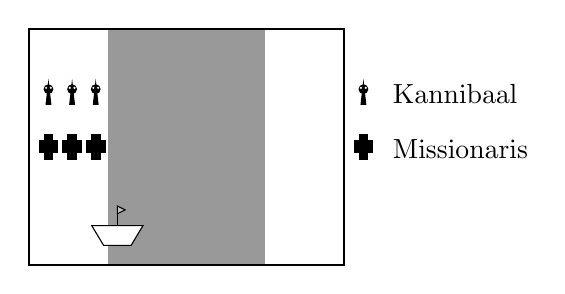
\begin{tikzpicture}
\def\ss{1.3247};%silver section is a catholic ratio
\def\cw{0.25};
\def\ch{\cw*\ss};
\fill[gray!80] (-1,-1.5) rectangle (1,1.5);
\draw[thick] (-2,-1.5) rectangle (2,1.5);
\filldraw[fill=white,draw=black] (-1.2,-1) -- (-0.55,-1) -- (-0.7,-1.25) -- (-1.05,-1.25) -- cycle;
\filldraw[fill=gray!50,draw=black] (-0.875,-0.85) -- (-0.875,-0.75) -- (-0.775,-.8) -- cycle;
\draw (-0.875,-1) -- (-0.875,-0.85);
\foreach\x in {0,0.3,0.6} {
  \fill (-1.75-0.25*\cw+\x,-0.5*\ch) rectangle (-1.75+0.25*\cw+\x,0.5*\ch);
  \fill (-1.75-0.5*\cw+\x,-0.25*\ch) rectangle (-1.75+0.5*\cw+\x,0.25*\ch);
  \fill (-1.75-0.15*\cw+\x,0.7-0.5*\ch) -- (-1.75+\x,0.7+0.5*\ch) -- (-1.75+0.15*\cw+\x,0.7-0.5*\ch) -- cycle;
  \fill (-1.75+\x,0.7+0.1*\ch) circle(0.25*\cw);
  \fill[white] (-1.78+\x,0.7+0.15*\ch) circle(0.06125*\cw);
  \fill[white] (-1.72+\x,0.7+0.15*\ch) circle(0.06125*\cw);
}
\fill (-1.75-0.25*\cw+4,-0.5*\ch) rectangle (-1.75+0.25*\cw+4,0.5*\ch);
\fill (-1.75-0.5*\cw+4,-0.25*\ch) rectangle (-1.75+0.5*\cw+4,0.25*\ch);
\fill (-1.75-0.15*\cw+4,0.7-0.5*\ch) -- (-1.75+4,0.7+0.5*\ch) -- (-1.75+0.15*\cw+4,0.7-0.5*\ch) -- cycle;
\fill (-1.75+4,0.7+0.1*\ch) circle(0.25*\cw);
\fill[white] (-1.78+4,0.7+0.15*\ch) circle(0.06125*\cw);
\fill[white] (-1.72+4,0.7+0.15*\ch) circle(0.06125*\cw);
\draw (2.5,0.7-0.1*\ch) node[anchor=west] {Kannibaal};
\draw (2.5,-0.1*\ch) node[anchor=west] {Missionaris};
\end{tikzpicture}
\caption{Begintoestand van het Missionaries \& Cannibals probleem}
\label{fig:missionariesAndCannibals}
\end{figure}
\section{Wat is een State-space?}
Een \termenglos{state-space}{De verzameling toestanden waarin een specifiek probleem zich kan bevinden. De toestanden dienen deterministisch en ondubbelzinnig uitgedrukt te worden.} is de verzameling van de verschillende staten (toestanden) waarin een probleem zich kan bevinden, waarbij de staat deterministisch en ondubbelzinnig uitgedrukt wordt. Daarnaast bevat een state-space ook een set \termenglos{productieregels}{Een set van regels (functies) die beschrijven onder welke omstandigheden men van een toestand in een andere toestand kan overgaan.}: condities om van de ene staat van het probleem naar een andere te gaan. Verder bezit een state-space ook een set \termenglos{begin sta(a)t(en)}{Een set toestanden die het begin van een specifiek probleem markeren.}, en een set voorwaarden waarbij het \termenglos{doel}{Een toestand van een specifiek probleem die we dienen te bereiken.} is bereikt (we het probleem dus opgelost hebben).
\paragraph{}
\begin{leftbar}
Hoe zouden we nu het Missionaries \& Cannibals probleem kunnen omzetten naar een statespace? Het enige wat we eigenlijk moeten weten is hoeveel missionarissen en cannibalen er aan \'e\'en van de twee oevers staan, en aan welke oever de boot ligt. Daarom introduceren we een notatie die er als volgt uit ziet: $\left\langle M,K,B\right\rangle$ hierbij stellen $M$ het aantal missionarissen, en $K$ het aantal kannibalen voor op de linkeroever. En schrijven we voor $B$, $l$ indien de boot zich op de linkeroever, en $r$ indien de boot zich op de rechteroever bevindt. De begintoestand noteren we dus als $\left\langle3,3,l\right\rangle$. Het doel is logischerwijs: $\left\langle0,0,r\right\rangle$.
\paragraph{}
Zoals reeds eerder vermeld, is dit probleem gebonden aan enkele voorwaarden. Zo mogen er nooit meer kannibalen dan missionarissen op \'e\'en van de oevers aanwezig zijn, tenzij er zich geen missionarissen op deze oever bevinden. Dit vertaald zich naar twee regels die we hieronder beschrijven:
\begin{equation}
\left\langle M,K,B\right\rangle\mbox{ is geldig}\Leftrightarrow\left\{
\begin{array}{cl}
M=0\vee M\geq K&\mbox{\{Linker oever\}}\\
\wedge\\
M=3\vee M\leq K&\mbox{\{Rechter oever\}}
\end{array}\right.
\end{equation}
\paragraph{}
Welke productieregels defini\"eren we? Indien de boot links staat dienen we minstens \'e\'en en maximum twee personen over te zetten. Omgekeerd indien de boot aan de rechter oever ligt, dienen we \'e\'en of twee personen aan de linkerover toe te voegen. Indien we deze regels formaliseren, bekomen we volgende regels:
\begin{equation}
\left\{\begin{array}{rcl|l}
\left\langle M,K,l\right\rangle&\Rightarrow&\left\langle M-\delta_m,K-\delta_k,r\right\rangle&\delta_m,\delta_k\in\left\{0,1,2\right\}\wedge1\leq\delta_m+\delta_k\leq 2\\
\left\langle M,K,r\right\rangle&\Rightarrow&\left\langle M+\delta_m,K+\delta_k,l\right\rangle&\delta_m,\delta_k\in\left\{0,1,2\right\}\wedge1\leq\delta_m+\delta_k\leq 2\\
\end{array}\right.
\end{equation}
\end{leftbar}
\section{Wat zijn de keuzes bij een State-space?}
\label{ss:stateSpaceTradeOffs}
Er zijn verschillende keuzes te maken:
\begin{itemize}
 \item Welke regel passen we eerst toe (proberen we eerst uit)
 \item Zoeken we in een boom of een graaf
 \item Zijn we op zoek naar de optimale oplossing, of is een oplossing voldoende
 \item Kunnen we het probleem opdelen in verschillende deelproblemen
 \item Zoeken we vooruit of achteruit
\end{itemize}
\paragraph{}
Indien we voor een optimale oplossing kiezen moeten we bijhouden wat de geaccumuleerde kost (zie \ref{ss:optimalSearch}) precies inhoud.
\paragraph{}
Indien we een keuze maken tussen \termenglos{voorwaarts redeneren}{Een strategie bij het zoeken door een state-space, waarbij we vanuit een begintoestand het doel proberen te bereiken.} of \termenglos{achterwaarts redeneren}{Een strategie bij het zoeken door een state-space, waarbij we vanuit het doel een begintoestand proberen te bereiken door productieregels omgekeerd toe te passen.}, moeten we vooral kijken naar de volgende criteria:
\begin{itemize}
 \item Zijn de regels achterwaarts te construeren: (bij schaken kan je niet achteruit denken)
 \item \termenglos{Branching factor}{Het gemiddelde aantal toestanden die direct afgeleid kunnen worden uit een toestand.}: het gemiddelde aantal staten die direct afgeleid kan worden uit een staat.
 \item Aantal begintoestanden ten opzichte van het aantal eindtoestanden
 \item Een achterwaartse redenering kan meestal meer zijn keuzes verklaren
\end{itemize}
Een andere mogelijkheid is \termenglos{Middle-out reasoning}{Een strategie bij het zoeken door een state-space, waarbij we vanuit een toestand zowel een begintoestand en doel trachtten te bereiken.} waarbij vanuit een bepaalde staat naar het doel en een begin gegraven wordt.
\paragraph{}
\begin{leftbar}
Het is duidelijk dat de het Missionaries \& Cannibals probleem een graaf is, immers kunnen we indien we een bepaalde transactie gedaan hebben, telkens deze ongedaan maken door de overgezette personen terug over te zetten. Op zich zijn we niet op zoek naar de kortste oplossing. We kunnen echter wel oplossingen genereren die heel veel redundant werk doen (door bijvoorbeeld een aantal keer op stappen terug te keren). Omdat dit probleem relatief simpel is, is het niet verder op te delen. We kunnen het probleem ook trachtten op te lossen door achterwaarts vanuit de oplossing te redeneren. Maar deze oplossing is eigenlijk volledig identiek. Op figuur \ref{fig:missionariesAndCannibalsGraph} wordt de graaf weergegeven die alle toestanden van het probleem weergeeft.
\end{leftbar}
\begin{figure}[htb]
\centering
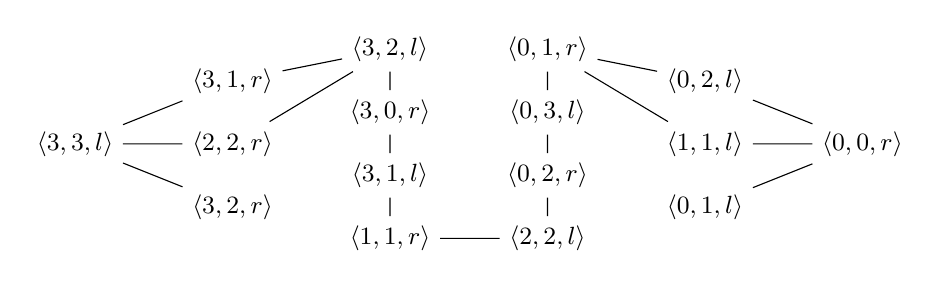
\begin{tikzpicture}
\def\dx{2};
\def\dy{-0.8};
\node (S33l) at (0,0) {\small$\left\langle 3,3,l\right\rangle$};
\node (S32r) at (\dx,\dy) {\small$\left\langle 3,2,r\right\rangle$};%dead
\node (S22r) at (\dx,0) {\small$\left\langle 2,2,r\right\rangle$};
\node (S31r) at (\dx,-\dy) {\small$\left\langle 3,1,r\right\rangle$};
\node (S32l) at (2*\dx,-1.5*\dy) {\small$\left\langle 3,2,l\right\rangle$};
\node (S30r) at (2*\dx,-0.5*\dy) {\small$\left\langle 3,0,r\right\rangle$};
\node (S31l) at (2*\dx,0.5*\dy) {\small$\left\langle 3,1,l\right\rangle$};
\node (S11r) at (2*\dx,1.5*\dy) {\small$\left\langle 1,1,r\right\rangle$};
\node (S22l) at (3*\dx,1.5*\dy) {\small$\left\langle 2,2,l\right\rangle$};
\node (S02r) at (3*\dx,0.5*\dy) {\small$\left\langle 0,2,r\right\rangle$};
\node (S03l) at (3*\dx,-0.5*\dy) {\small$\left\langle 0,3,l\right\rangle$};
\node (S01r) at (3*\dx,-1.5*\dy) {\small$\left\langle 0,1,r\right\rangle$};
\node (S01l) at (4*\dx,\dy) {\small$\left\langle 0,1,l\right\rangle$};
\node (S11l) at (4*\dx,0) {\small$\left\langle 1,1,l\right\rangle$};
\node (S02l) at (4*\dx,-\dy) {\small$\left\langle 0,2,l\right\rangle$};
\node (S00r) at (5*\dx,0) {\small$\left\langle 0,0,r\right\rangle$};
\draw (S33l) -- (S32r);
\draw (S33l) -- (S22r) -- (S32l);
\draw (S33l) -- (S31r) -- (S32l) -- (S30r) -- (S31l) -- (S11r) -- (S22l) -- (S02r) -- (S03l) -- (S01r) -- (S02l) -- (S00r);
\draw (S01r) -- (S11l) -- (S00r);
\draw (S01l) -- (S00r);
% \node (S00l) at (0,0) {$\left\langle 0,0,l\right\rangle$};
% \node[draw=black,rectangle] (S00r) at (4*\dx,0) {$\left\langle 0,0,r\right\rangle$};
% \node (S01l) at (\dx,0) {$\left\langle 0,1,l\right\rangle$};
% \node (S01r) at (5*\dx,0) {$\left\langle 0,1,r\right\rangle$};
% \node (S02l) at (2*\dx,0) {$\left\langle 0,2,l\right\rangle$};
% \node (S02r) at (6*\dx,0) {$\left\langle 0,2,r\right\rangle$};
% \node (S03l) at (3*\dx,0) {$\left\langle 0,3,l\right\rangle$};
% \node (S03r) at (7*\dx,0) {$\left\langle 0,3,r\right\rangle$};
% \node (S30l) at (0,3*\dy) {$\left\langle 3,0,l\right\rangle$};
% \node (S30r) at (4*\dx,3*\dy) {$\left\langle 3,0,r\right\rangle$};
% \node (S31l) at (\dx,3*\dy) {$\left\langle 3,1,l\right\rangle$};
% \node (S31r) at (5*\dx,3*\dy) {$\left\langle 3,1,r\right\rangle$};
% \node (S32l) at (2*\dx,3*\dy) {$\left\langle 3,2,l\right\rangle$};
% \node (S32r) at (6*\dx,3*\dy) {$\left\langle 3,2,r\right\rangle$};
% \node (S33r) at (7*\dx,3*\dy) {$\left\langle 3,3,r\right\rangle$};
% \node (S11l) at (\dx,\dy) {$\left\langle 1,1,l\right\rangle$};
% \node (S22l) at (2*\dx,2*\dy) {$\left\langle 2,2,l\right\rangle$};
% \node (S11r) at (5*\dx,\dy) {$\left\langle 1,1,r\right\rangle$};
% \node (S22r) at (6*\dx,2*\dy) {$\left\langle 2,2,r\right\rangle$};
% 
% \draw (S33l) .. controls ++(0,-\dy) and ++(0,-\dy) .. (S32r);
% \draw (S33l) .. controls ++(0,-\dy) and ++(0,-\dy) .. (S31r) -- (S32l) -- (S30r) -- (S31l) -- (S11r) -- (S22l) -- (S02r) -- (S03l) -- (S01r) -- (S11l) -- (S00r);
% \draw (S33l) -- (S22r) -- (S32l);
% \draw (S01r) -- (S02l) -- (S00r);
\end{tikzpicture}
\caption{Graaf van de verschillende toestanden}
\label{fig:missionariesAndCannibalsGraph}
\end{figure}